\documentclass{standalone}
\usepackage{tikz}
\usepackage{graphicx}
\usetikzlibrary{arrows.meta, positioning}
\begin{document}
\begin{tikzpicture}
    \node[anchor=south west, inner sep=0] (img) at (0,0)
        {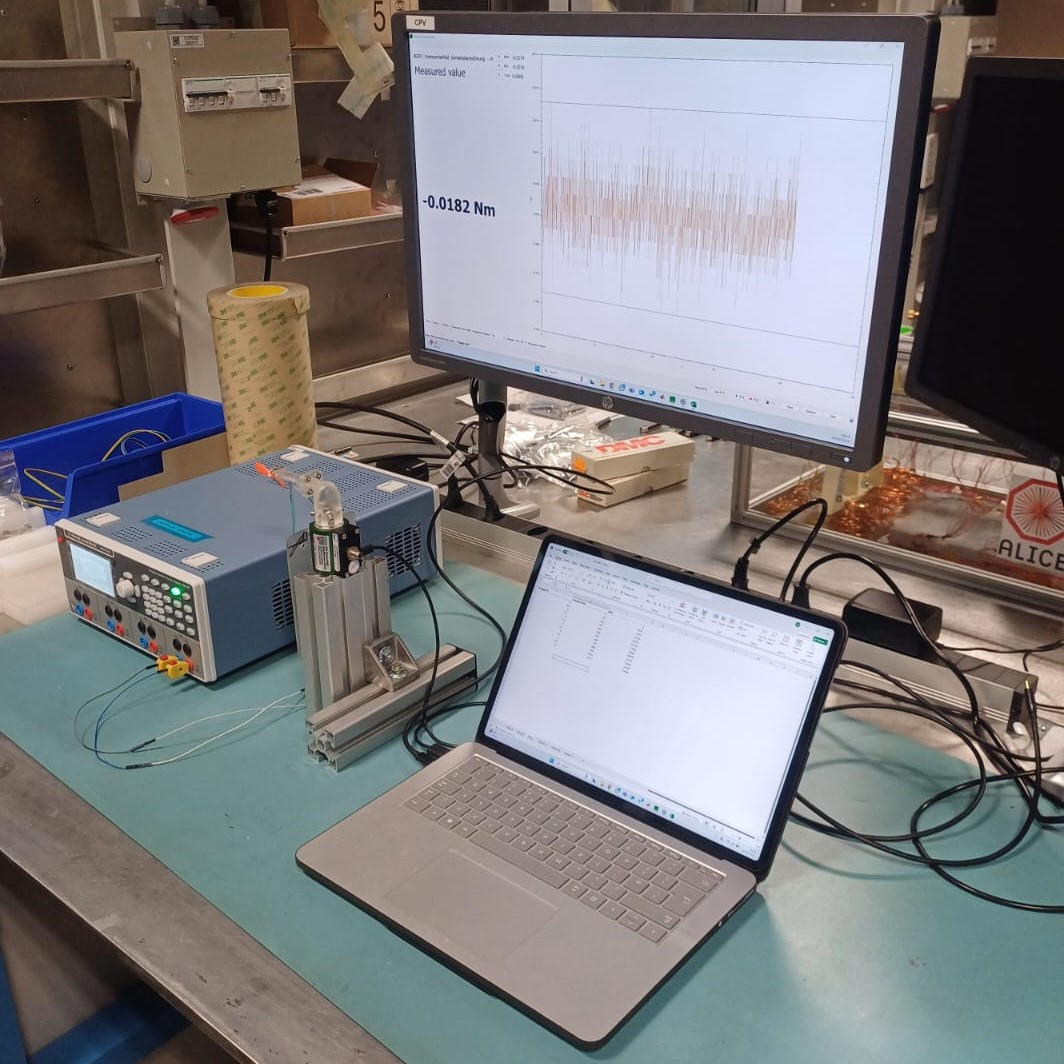
\includegraphics[width=10cm]{test_setup_thrust.jpg}};
    \begin{scope}[
        x={(img.south east)},
        y={(img.north west)}
    ]
    \tikzset{
        lbl/.style={
            fill=white,
            draw=red,
            thick,
            rounded corners=2pt,
            font=\small,
            inner sep=3pt,
            align=center,
        },
        arr/.style={
            red, thick,
            -latex,
        },
    }
    % Power supply
    \node[lbl] (lblPower) at (0.12, 0.61) {Power supply};
    \draw[arr] (lblPower.south) -- (0.12, 0.5);
    % DC Motor & Propeller  — two lines
    \node[lbl] (lblProp) at (0.25, 0.7) {DC Motor \\ \& Propeller};
    \draw[arr] (lblProp.south) -- (0.25, 0.57);
    % Torquemeter
    \node[lbl] (lblTorsion) at (0.5, 0.58) {Torquemeter};
    \draw[arr] (lblTorsion.south) -- (0.32, 0.5);
    % Test rig
    \node[lbl] (lblRig) at (0.20, 0.30) {Test rig};
    \draw[arr] (lblRig.north) -- (0.32, 0.42);
    \end{scope}
\end{tikzpicture}
\end{document}